\chapter{Método Runge-Kutta de Dormand y Prince Localmente Linealizado para EDOs de
dimensiones no pequeñas}\label{chapter:lldp}
En el Capítulo \ref{chapter:exp-int-and-ll-methods} se presentó la Aproximación Lineal Local de Orden Superior. Esta aproximación consiste en descomponer la solución de la ecuación diferencial original como la suma de las soluciones de dos ecuaciones diferenciales auxiliares, una lineal y la no lineal. En el Capítulo \ref{chapter:solve-non-smal-lineal-eq} se propusieron y utilizaron las aproximaciones Krylov-Padé para resolver la ecuación diferencial lineal auxiliar. En este capítulo se utilizará el método Runge-Kutta de Dormand y Prince para aproximar la solución de la ecuación diferencial no lineal auxiliar. Combinando estas aproximaciones se obtienen Método Runge-Kutta de Dormand y Prince Localmente Linealizado para EDOs de dimensiones no pequeñas.

Sin pérdida de generalidad consideremos el PVI autónomo $d$-dimensional
\begin{equation}\label{syst}
\frac{dx}{dt}=f(x), \; t\in[t_0,T],\end{equation}
\begin{equation}\label{systcond}
x(t_0)=x_0,
\end{equation}donde $f$ es una función diferenciable en una vecindad
$\mathfrak{D}$ del conjunto $\{x(t):t\in [t_0,T]\}$ de $\mathbb{R}^{d}$. Se asumen condiciones de Lipschitz y suavidad en la función $f$ para asegurar una solución única de esta ecuación en $\mathfrak{D}$.

\section{Fórmulas embebidas}

Sea $\left( t\right) _{h}=\left\{ t_{n}:n=0,1,\ldots ,N\right\}$ una discretización temporal con un tamaño de paso máximo $h$ definido como una secuencia de tiempos que satisfacen las condiciones $t_{0}<t_{1}<\cdots <t_{N}=T$, donde $h_{n}=t_{n+1}-t_{n}\leq h$ para $n=0,\ldots,N-1$.

Consideremos las fórmulas de Runge-Kutta localmente linealizadas de Dormand y Prince
\begin{equation} \label{lldis}
    z_{n+1}\,=\,z_n+u_s+h_n \sum_{j=1}^{s}b_j \kt_j \,\,\, \text{and} \,\,\, \
    \widehat{z}_{n+1}\,=\, z_n+u_s+h_n \sum_{j=1}^{s}\widehat{b}_j \kt_j
\end{equation}
introducidas en \cite{Jimenez14AMC} para aproximar la solución $x$ de (\ref{syst})-(\ref{systcond}) en $t_{n+1}$, para $n=0,\ldots,N -1$, donde s = 7 es el número de etapas,
\begin{equation*}
u_j=L\me{c_j M_n h_n}r,
\end{equation*}
\begin{equation*}
\kt_j = f\left( z_n+u_j+h_n \sum_{i=1}^{j-1}a_{j,i}\kt_i \right) - f( z_n) - f_x(z_n)u_j,
\end{equation*}
con $\kt_1 \equiv 0$, siendo $f_x$ la matriz jacobiana de $f$ y $a_{j,i}$, $b_j$, $\widehat{b}_j$ los coeficientes de Runge-Kutta de Dormand y Príncipe definido en la Tabla \ref{ButcherTabla}. Aquí,
\begin{equation*}
    M_{n}=\left[
    \begin{array}{cc}
        f_{x}(z_{n}) & f(z_{n}) \\
        0_{1\times d} & 0
    \end{array}
    \right] \in \mathbb{R}^{(d+1)\times (d+1)},
\end{equation*}
$ L=[I_d \;\; 0_{d\times 1}] $ and $r=[0_{1\times d}\;\; 1]^T$. Las fórmulas embebidas (\ref{lldis}) son instancias particulares de una clase más general de métodos de linealización local de alto orden propuestos en \cite{Jimenez13}.

\begin{table}[h]
	\caption{Tabla de coeficientes para las fórmulas embebidas de Dormand y Prince} \label{ButcherTabla}
	\begin{center}
		\begin{tabular}{ l@{\vrule height 5pt depth 10pt width 0pt}|lllllll}
			$0$ & \\
			$\frac{1}{5}\quad$ & $\frac{1}{5}$ \\
			$\frac{3}{10}\quad$ & $\frac{3}{40}$ & $\frac{9}{40}$ \\
			$\frac{4}{5}\quad$ & $\frac{44}{45}$ & $-\frac{56}{15}$ & $\frac{32}{9}$ \\
			$\frac{8}{9}\quad$ & $\frac{19372}{6561}$ & $-\frac{25360}{2187}$ & $\frac{64448}{6561}$ & $-\frac{212}{729}$ \\
			$1\quad$ & $\frac{9017}{3168}$ & $-\frac{355}{33}$ & $\frac{46732}{5247}$ & $\frac{49}{176}$
			& $-\frac{5103}{18656}$ \\
			$1\quad$ & $\frac{35}{384}$ & $0$ & $\frac{500}{1113}$ & $\frac{125}{192}$
			& $-\frac{2187}{6784}$ & $\frac{11}{84}$ \\
			\hline
			$\widehat{y}$ & $\frac{5179}{57600}$ & $0$ & $\frac{7571}{16695}$ & $\frac{393}{640}$
			& $-\frac{92097}{339200}$ & $\frac{187}{2100}$ & $\frac{1}{40}$
			\rule[-0.3cm]{0cm}{0.8cm} \\
			$y$ & $\frac{35}{384}$ & $0$ & $\frac{500}{1113}$ & $\frac{125}{192}$
			& $-\frac{2187}{6784}$ & $\frac{11}{84}$ & $0$
		\end{tabular}
	\end{center}
\end{table}

Las aproximaciones Krylov-Padé propuestas en el capítulo anterior serán utilizadas para aproximar los términos $u_j$ que aparecen en (\ref{lldis}). Además, para aproximar eficientemente los cinco términos $u_j$ correspondientes a los cinco únicos $c_j$ distintos de cero que según la Tabla \ref{ButcherTabla} aparecen en las fórmulas (\ref{lldis}), se utilizará combinación conveniente de la invarianza ante escalado de la base ortonormal de los subespacios de Krylov, la propiedad de flujo del operador exponencial y el Teorema 1 en~\cite{sidje1998expokit}. De hecho, con la matriz de Hessenberg superior $H^*_\mf$ resultante del algoritmo \ref{alg:Arnoldi} para $\mathcal{K}_\mf(h_nf_x,f)$, se obtiene la matriz de Hessenberg $H_\mf=H^*_\mf/h_n$ correspondiente a $\mathcal{K}_\mf(f_x,f)$, por lo que la exponencial de la matriz particionada
\begin{equation}
    \overline{H} = \left[\begin{array}{cccc}
    H_\mf & e_1 & 0_{\mf\times 1} & 0_{\mf\times 1}\\
    0_{1\times\mf} & 0 & 1 & 0\\
    0_{1\times\mf} & 0 & 0 & 1\\
    0_{1\times\mf} & 0 & 0 & 0
    \end{array}\right] \label{hhat}
\end{equation}
es calculada obteniéndose
\begin{equation}
    \me{\tau\overline{H}} = \left[\begin{array}{cccc}
    \me{\tau H_m} & \tau\phi_1(\tau H_m)e_1 & \tau^{2}\phi_2(\tau H_m)e_1 &
    \tau^{3}\phi_3(\tau H_m)e_1 \\
    & 1 & \tau & \frac{\tau^{2}}{2}\\
    &  & 1 & \tau \\
    &   &   & 1 \\
    \end{array}\right]\;. \label{phi_hhat}
\end{equation}
En particular, con $\gamma=\frac{1}{90}$, es calculada la matriz particionada $E_\gamma=\me{\gamma h_n\overline{H}}$, donde $\frac{1}{ 90}$ es el máximo común divisor de los coeficientes de Runge-Kutta $\frac{1}{5},\frac{3}{10},\frac{4}{5},\frac{8}{9} ,1$ de la Tabla \ref{ButcherTabla}. Usando la propiedad de flujo del operador exponencial se obtiene

\begin{align}
    E_{2/90}& =E_{1/90}E_{1/90} & E_{4/90}& =E_{2/90}E_{2/90}  \notag \\
    E_{8/90}& =E_{4/90}E_{4/90} & E_{16/90}& =E_{8/90}E_{8/90}  \notag \\
    E_{32/90}& =E_{16/90}E_{16/90} & E_{80/90}& =E_{32/90}E_{16/90}E_{32/90}
    \label{flow} \\
    E_{1/10}& =E_{8/90}E_{1/90} & E_{1/5}& =E_{1/10}E_{1/10}  \notag \\
    E_{2/5}& =E_{1/5}E_{1/5} & E_{4/5}& =E_{2/5}E_{2/5}  \notag \\
    E_{3/10}& =E_{1/10}E_{1/5} & E_{1}& =E_{4/5}E_{1/5}\;,  \notag
\end{align}
con lo cual las cinco matrices requeridas $E_{c_j}$ son obtenidas. Como la exponencial no puede ser calculada de forma exacta ene caso general se aproximará utilizando Padé como se explica en el Capítulo \ref{chapter:solve-non-smal-lineal-eq} obteniéndose $\widetilde{E}_{c_j}$.

Por lo tanto, utilizando la aproximación Krylov-Padé (\ref{eq:kp_aprox}) y (\ref{flow}) obtenemos las aproximaciones para cada $u_j$
\begin{eqnarray}
    \frac{1}{5}h_n\varphi_1\left(\frac{1}{5}h_n f_x\right)f & \approx & \beta   V_{\mf}\; [\widetilde{E}_{\frac{1}{5}}]_{12}\;  + \beta \hf_{\mf+1,\mf}e_\mf^T\; [\widetilde{E}_{\frac{1}{5}}]_{13}\;  v_{\mf+1} \notag \\
    \frac{3}{10}h_n\varphi_1\left(\frac{3}{10}h_n f_x\right)f & \approx & \beta   V_{\mf}\; [\widetilde{E}_{\frac{3}{10}}]_{12}\;  + \beta \hf_{\mf+1,\mf}e_\mf^T\; [\widetilde{E}_{\frac{3}{10}}]_{13}\;  v_{\mf+1} \notag \\
    \frac{4}{5}h_n\varphi_1\left(\frac{4}{5}h_n f_x\right)f & \approx & \beta   V_{\mf}\; [\widetilde{E}_{\frac{4}{5}}]_{12}\;  + \beta \hf_{\mf+1,\mf}e_\mf^T\; [\widetilde{E}_{\frac{4}{5}}]_{13}\;  v_{\mf+1} \label{phi_appox} \\
    \frac{8}{9}h_n\varphi_1\left(\frac{8}{9}h_n f_x\right)f & \approx & \beta   V_{\mf}\; [\widetilde{E}_{\frac{8}{9}}]_{12}\;  + \beta \hf_{\mf+1,\mf}e_\mf^T\; [\widetilde{E}_{\frac{8}{9}}]_{13}\;  v_{\mf+1} \notag \\
    h_n\varphi_1(h_n f_x)f & \approx &  \beta V_{\mf}\; [\widetilde{E}_1]_{12}\;  + \beta\hf_{\mf+1,\mf}e_\mf^T\; [\widetilde{E}_1]_{13}\;  v_{\mf+1}, \notag
\end{eqnarray}
donde $[\widetilde{E}_{c_j}]_{ik}$ denota la submatriz $i,k$ de la matriz particionada $\widetilde{E}_{c_j}$, $V_m$ es la matriz con base ortonormal de $\mathcal{K}_ \mf(f_x,f)$ ya calculado por el Algoritmo \ref{alg:Arnoldi} para $\mathcal{K}_\mf(h_nf_x,f)$, y $\beta=\nnorm{\nnorm{f} }_2$.

Utilizando la aproximación $(\mf , \pf ,\qf , k)$-Krylov-Padé (\ref{eq:kp_aprox}) para $u_j$ en las fórmulas embebidas (\ref{lldis}), obtenemos la Fórmulas de Runge-Kutta linealizadas localmente
\begin{equation}  \label{LLDPK scheme}
    y_{n+1}\,=\,y_n+\widetilde{u}_s+h_n \sum_{j=1}^{s}b_j \widetilde{\kt}_j \,\,\, \text{and} \,\,\, \
    \widehat{y}_{n+1}\,=\, y_n+\widetilde{u}_s+h_n \sum_{j=1}^{s}\widehat{b}_j \widetilde{\kt}_j,
\end{equation}
para integrar PVI de grandes dimensiones, donde
\begin{equation*}
    \widetilde{\kt}_j = f\left( y_n+\widetilde{u}_j+h_n \sum_{i=1}^{j-1}a_{j,i}\widetilde{\kt}_i \right) - f( y_n) - f_x(y_n)\widetilde{u}_j.
\end{equation*}
y $\widetilde{\kt}_1=0$, son $a_{j,i}$, $b_j$, $\widehat{b}_j$ los coeficientes de Runge-Kutta de  Dormand y Prince definidos en la Tabla \ref{ButcherTabla}.

Es importante destacar que, a diferencia de otros integradores exponenciales de alto orden, las fórmulas embebidas (\ref{LLDPK scheme}) involucran la aproximación de un solo vector de tiempo de función phi. En efecto, mientras que los integradores exponenciales en general requieren de aproximar varios términos de la forma $\tau^k \varphi_k(\tau A_k)b_k$ con más de un valor de $k$, las fórmulas embebidas (\ref{LLDPK scheme}) solo requieren la aproximación de la acción de una sola función phi sobre un único vector $\tau \varphi_1(\tau A_1)b_1$. Como se ha explicado anteriormente, las cinco aproximaciones $\widetilde{u}_j$ a los términos distintos de cero $c_jh_n\varphi_1(c_jh_nf_x)f$ que aparecen en (\ref{LLDPK scheme}) se calculan eficientemente en cada paso de integración por medio de solo una aproximación por un subespacio de Krylov que se construye mediante el algoritmo \ref{alg:Arnoldi} y solo una exponencial matricial mediante el método de Padé.

El siguiente teorema trata sobre la velocidad de convergencia de las fórmulas embebidas (\ref{LLDPK scheme}). Con este propósito, estas fórmulas se reescriben como
\begin{equation*}
    y_{n+1}=y_{n}+\digamma (y_{n};h_{n})\text{ \ \ \ \ y \ \ \ \ }\widehat{y}_{n+1}=y_{n}+\widehat{\digamma }(y_{n};h_{n}).
\end{equation*}


\begin{theorem}\label{theorem:lldp-convergence}
	Se $x$ solución del PVI (\ref{syst})-(\ref{systcond}) con campo vectorial $f$ seis veces continuamente diferenciable en con conjunto compacto $\mathfrak{K} \subset \mathfrak{D}$. Entonce, las formular Runge-Kutta Localmente Linealizadas (\ref{LLDPK scheme}) tienen error de truncamiento local
	\[\lvert\lvert x(t_{n+1}) - x(t_n) - \digamma(x(t_n);h_n) \rvert\rvert_2 \leq Kh_n^{\mathrm{min}\left\{ \mf+2,\pf+\qf+1 \right\}}+C h_n^{6}  \]
	\[\lvert\lvert x(t_{n+1}) - x(t_n) - \widehat{\digamma }(x(t_n);h_n) \rvert\rvert_2 \leq Kh_n^{\mathrm{min}\left\{ \mf+2,\pf+\qf+1 \right\}}+C h_n^{5}  \]
	y erro global
	\[ \lvert\lvert x(t_{n+1}) - y_{n+1} \rvert\rvert_2 \leq M h^{\mathrm{min}\left\{5,\mf+1,\pf+\qf \right\}} \]
	\[ \lvert\lvert x(t_{n+1}) - \widehat{y}_{n+1} \rvert\rvert_2 \leq M h^{\mathrm{min}\left\{ 4,\mf+1,\pf+\qf \right\}} \]
	$\forall t_{n+1},t_n\in(t)_h$ y $h$ suficientemente pequeña, donde  $K,C,M$ son constantes positivas.
\end{theorem}
\emph{Demostración} Utilizando el Teorema~\ref{theorem:Krylov-bound}, se tiene
\begin{equation}\label{proof:ErrorLinearODE}
\nnorm{\nnorm{ u_j-K_{\mf,k}^{\pf,\qf}\left(c_j h_n,f_x , f \right) }}_2 =  \nnorm{\nnorm{c_jh_n\varphi_1(c_jh_nf_x)f - K_{\mf,k}^{\pf,\qf}\left(c_j h_n, f_x , f \right) }}_2 \le Kh_n^{\mathrm{min}\left\{ \mf+2,\pf+\qf+1 \right\}},
\end{equation}
con $j=1,\ldots,7$, donde $K$ es una constante positiva. Dado que $z_{n+1} = y_n + u_7$ es la solución exacta de la EDO lineal $dz/dt=f(y_n)+f_x(y_n)(z-y_n)$ resultante de la linealización local de la ecuación~(\ref{syst}) en $t_n$ con la condición inicial $z(t_n)=y_n$ y los errores de truncamiento local de las fórmulas embebidas de Runge-Kutta de Dormand y Prince son 6 y 5, los errores de truncamiento local y global del Las fórmulas de Runge-Kutta localmente linealizadas (\ref{LLDPK scheme}) se derivan directamente del Teorema 15 en~\cite{Jimenez13} y (\ref{proof:ErrorLinearODE}). $\Box$\\

Claramente, según este resultado, las fórmulas embebidas Runge-Kutta localmente linealizadas (\ref{LLDPK scheme}) preservan la velocidad de convergencia de las fórmulas embebidas clásicas Runge-Kutta de Dormand y Prince si las desigualdades $\mf+1 \ge 5 $ y $\pf+\qf \ge 5$ se cumplen. Además, al igual que las fórmulas embebidas para pequeños PVI y otros integradores de tipo exponencial, las nuevas fórmulas embebidas (\ref{LLDPK scheme}) son capaces de integrar PVI lineales tan precisos como sea necesario independientemente de la dimensionalidad y \textit{stiffness} de las ecuaciones. Sin embargo, dado que, por construcción, las fórmulas (\ref{LLDPK scheme}) usan las fórmulas originales de Runge-Kutta de Dormand y Prince para resolver una ecuación auxiliar no lineal (ver detalles en \cite{Jimenez13, Jimenez14AMC}), las fórmulas (\ref{LLDPK scheme}) no están diseñadas para integrar PVI \textit{stiff} en general. De esta forma, las fórmulas propuestas (\ref{LLDPK scheme}) pretenden aproximar la solución de PVI grandes para los que la principal fuente de \textit{stiffness} surge de la linealización de la ecuación no lineal en consideración. Estos son precisamente la mayoría de los grandes PVI resultantes de la discretización espacial de las EDP que modelan procesos físicos, biofísicos y físico-químicos conocidos.
\begin{table}[h]
	\caption{ Valores de los coeficientes $\alpha _{i,j}$ en las fórmulas continuas (\ref{continuousLLRK45}) \newline \label{Table continuous RK}}
	\centering
	\begin{tabular}{ccccc}
		\hline
		$j\setminus i$ & $1$ & $2$ & $3$ & $4$ \\
		\hline
		$1$ & $1$ & $-183/64$ & $37/12$ & $-145/128$ \\
		$2$ & $0$ & $0$ & $0$ & $0$ \\
		$3$ & $0$ & $1500/371$ & $-1000/159$ & $1000/371$ \\
		$4$ & $0$ & $-125/32$ & $125/12$ & $-375/64$ \\
		$5$ & $0$ &	$9477/3392$ & $-729/106$ & $25515/6784$ \\
		$6$ & $0$ &	$-11/7$ & $11/3$ & $-55/28$ \\
		$7$ & $0$ & $3/2$ & $-4$ & $5/2$ \\
		\hline
	\end{tabular}
\end{table}
Cuando se requiere la solución en un conjunto denso de instantes de tiempo entre dos pasos de integración consecutivos, normalmente se utilizan fórmulas continuas para proceder con un costo computacional mínimo (consulte, por ejemplo, la Sección II.6 en \cite{hairer1993solving}). Regularmente, estas fórmulas continuas se construyen mediante una interpolación polinomial de las fórmulas de integración entre dos pasos de integración consecutivos $t_{n},t_{n+1}\in $ $ t_{h}$. Mediante una simple combinación de las fórmulas embebidas (\ref{LLDPK scheme}) con las fórmulas continuas de Runge-Kutta de Dormand y Prince dadas en \cite{hairer1993solving}, se obtiene la siguiente fórmula continua de $7$ etapas
\begin{equation}
    y(t_{n}+\theta h_{n})=y_n+\widetilde{u}(\theta
    h_{n})+h_{n}\sum_{j=1}^{7}b_{j}(t_{n}+\theta h_{n})\widetilde{\kt}_{j}\
    ,\ \ 0<\theta <1,  \label{continuousLLRK45}
\end{equation}%
 para todo $t_{n} \in $ $\left( t\right) _{h}$, donde
\begin{equation*}
    \widetilde{u}(\theta h_{n}) = K_{\mf,k}^{\pf,\qf}\left(h_n\theta, f_x , f \right)
\end{equation*}
    es el vector $d$-dimensional,
\begin{equation*}
    b_{j}(\delta )=\sum\limits_{i=1}^{4}\alpha _{i,j}\delta ^{i}
\end{equation*}
es un polinomio con coeficientes $\alpha _{i,j}$, y la función $\widetilde{\kt}_{j}$ se define como en (\ref{LLDPK scheme}). Los coeficientes $\alpha _{i,j}$, definidos en
Tabla \ref{Table continuous RK}, coinciden con las de la
fórmula continua de Runge-Kutta implementada en el código de Matlab ode$45$. Para la fórmula continua (\ref{continuousLLRK45}) se pueden definir dos salidas densas convenientes. La primera, de 4 elementos, incluye los pares $(t_{n}+\theta h_{n},y(t_{n}+\theta h_{n}))$ correspondientes a los cuatro $\theta = c_j $, con $0<c_j<1$, para la cual ya se han calculado las aproximaciones $\widetilde{u}_j$ en (\ref{LLDPK scheme}). El segundo conjunto se define con los doce valores
$\{\frac{1}{90},\frac{2}{90},\frac{4}{90},\frac{8}{90},\frac{1}{10},\frac {16}{90},c_2,c_3,\frac{32}{90},\frac{2}{5},c_4,c_5\}$ de $\theta$ para las cuales las matrices $E_\theta$ en (\ref{flow}) fueron calculados. En este caso, $\widetilde{u}(\theta h_{n})$ debe evaluarse en los ocho valores de $\theta \ne c_j$, pero sin requerir alguna nueva aproximación del subespacio de Krylov.

Antes de concluir esta sección es importante destacar que las fórmulas incrustadas (\ref{LLDPK scheme}) como implementación numérica de las fórmulas incrustadas (\ref{lldis}) también pertenecen a la clase general de métodos de linealización local de alto orden de \cite{Jimenez13}. Además, tenga en cuenta que, simplemente reemplazando en (\ref{LLDPK scheme}) los coeficientes de la tabla \ref{ButcherTabla} por otros correspondientes a un par diferente de fórmulas de Runge-Kutta explícitas incrustadas con etapas $s$, un nuevo incrustado localmente linealizado Las fórmulas de Runge-Kutta se obtienen directamente para IVP grandes. La tasa de convergencia de tales nuevas fórmulas se obtiene, como en la demostración del Teorema \ref{theorem:lldp-convergence}, simplemente combinando el Teorema 15 en~\cite{Jimenez13} y el Teorema \ref{theorem:Krylov-bound}. Además, si los coeficientes de Runge-Kutta $c_i$ de las nuevas fórmulas admiten un máximo común divisor $\gamma$ entonces, un procedimiento similar al descrito en (\ref{flow}) puede seguirse para calcular los diferentes términos $u_j$ de manera eficiente.

\section{Esquemas con tamaño de paso fijo y dimensión de Krylov variable}\label{section:lldp-fix-step}

Las nuevas fórmulas embebidas (\ref{LLDPK scheme}) introducidas en la sección anterior para integrar PVI de grandes dimensiones
dependen de valores no especificados para la dimensión Krylov $\mf$ y el orden Padé $(\pf ,\qf)$. En esta sección se propone una estrategia adaptativa para la estimación de valores adecuados para $\mf, \pf ,\qf$ en fórmulas (\ref{LLDPK scheme}) en cada paso de integración en una partición de tiempo uniforme.

\subsection{Selección de la dimensión de Krylov}

Similar al error relativo utilizado en la Sección \ref{section:num-sim-kp}, el error relativo en la aproximación \ref{LLDPK scheme} para $u_j$ está dado por
\begin{equation}
    \varepsilon_{K} = \left(\frac{1}{d}\sum\limits_{i=1}^{d} \left(\frac{\beta
        \hf_{\mf+1,\mf} e_{\mf}^T
        [\widetilde{E}_\mathfrak{c}]_{14} \rho^{[i]}}{ATol+ RTol\cdotp
        \rvert y_{n}^{[i]}\rvert}\right)^{2}\right)^{1/2},
    \label{errrel}
\end{equation}
donde $ATol$ y $RTol$ son las tolerancias absoluta y Relativa, $\mathfrak{c}=\maxx{c_j}$, $\rho = f_x v_{\mf+1}$ y $\beta=\nnorm{\nnorm{f}}_2$.

Después de la construcción de la base ortonormal del $\mf$-ésimo subespacio Krylov $\mathcal{K}_\mf(f_x,f)$, son posibles dos alternativas: $\varepsilon_{K}/\gamma_{K}< 1$ o al contrario, donde $\varepsilon_{K}$
es el error relativo~(\ref{errrel}) y $\gamma_{K}=0.005$ es un factor de seguridad.

En el caso de $\varepsilon_{K}/\gamma_{K}< 1$, se acepta la aproximación (\ref{phi_appox}) para $u_j$ y la nueva dimensión del subespacio de Krylov $\mathfrak{m}_{new}$ que se utilizará en el siguiente paso de integración se calcula mediante la fórmula
\begin{equation}\label{calcmnew}
    \mathfrak{m}_{new}= \maxx{\mf_{min}, \minn{\mf , \mf_{max} }},
\end{equation}
    donde $\mf_{min}$ y $\mf_{max}$ son los valores máximo y mínimo posibles para la dimensión del Krylov,
\begin{equation*}
    \mf = \left\lfloor \mf_{n} + \maxx{\fac_{max} , \minn{\fac_{min},
            \fac\cdot\Delta\mf} } \right\rfloor,
\end{equation*}
\begin{equation}
    \Delta\mf=\log(\varepsilon_{K}/\gamma_{K}) \label{delta_m}
\end{equation}
$\fac_{max}= -\frac{\mf_n}{4}$, $\fac_{min}= \frac{\mf_n}{3}$, $\fac=\frac{1}{\log( 2)}$, y $\left\lfloor \cdot \right\rfloor$ denota la función suelo(que devuelve el mayor entero menor o igual que un número real dado). De lo contrario, se rechaza la aproximación (\ref{phi_appox}) para $u_j$ para el $\mf_n$ dado y se estima un nuevo valor para la dimensión del subespacio de Krylov $\mf_{new}$ mediante (\ref{calcmnew}), pero con $\mf$ calculado por la expresión
\begin{equation*}
    \mf = \left\lceil \mf_{n} + \minn{\fac_{max} , \maxx{\fac_{min},
            \fac\cdot\Delta\mf} } \right\rceil,
\end{equation*}
donde $\fac_{max}= \maxx{ 1,\frac{\mf_{n}}{3} }$, $\fac_{min}= 1 $, $\fac=\frac{1}{\log (2)}$, y $\left\lceil \cdot \right\rceil$ denota la función techo(que devuelve el menor entero mayor o igual que un número real dado). Los vectores ortonormales extra $\{v_{\mf+1},\ldots,v_{\mf_{new}} \}$ correspondientes al $\mf_{new}$-ésimo subespacio de Krylov $\mathcal{K}_{\mf_{new}}(f_x,f)$son calculados a través del algoritmo \ref{alg:Arnoldiexpand}.
\begin{algorithm}[h!]
	\caption{Algoritmo de Arnoldi para expandir la base ortonormal $\{v_1,\ldots,v_{\mf} \}$ of the $\mf$-ésimo subespacio de Krylov $\mathcal{K}_{\mf}(A,b)=span\{b,Ab,\ldots,A^{\mf}b\}$ a la base ortonormal $\{v_1,\ldots,v_{\mf},\ldots,v_{\mf_{new}} \}$ del $\mf_{new}$-ésimo subespacio de Krylov ${\mathcal{K}_{\mf_{new}}(A,b)=span\{b,Ab,\ldots,A^{\mf_{new}}b\}}$}
    \label{alg:Arnoldiexpand}
	\KwIn{$A\in \mathbb{R}^{d\times d}$, $b\in \mathbb{R}^{d}$, $V_{\mf}\in \mathbb{R}^{d\times \mf}$, $H^*_{\mf}\in\mathbb{R}^{\mf\times \mf}$, $v_{\mf+1}\in \mathbb{R}^{d}$, $\hf_{\mf+1,\mf} \ge 0$, y la nueva dimensión $\mf_{new}$ xel subespacio de Krylov}
	\KwOut{$V_{\mf_{new}}=[v_1\,\cdots \,v_{\mf_{new}}]\in \mathbb{R}^{d\times \mf_{new}}$, matriz de Hessenberg superior $H^*_{\mf_{new}}=V_\mf^{\intercal} A V_{\mf_{new}} $, $v_{\mf_{new}+1}$,  $\hf_{\mf_{new}+1}$, $\mf_{new}$, $\mf_{cut}$, $breakdown$}
	Líneas 3-17 en el Algoritmo \ref{alg:Arnoldi}, pero reemplazando la línea 3 por \textbf{for} $j=\mf+1,\ldots,\mf_{new}$ \textbf{do}
\end{algorithm}
El estimador propuesto (\ref{calcmnew}) para $\mf_{new}$ es un refinamiento del considerado en el Algoritmo 3 de \cite{niesen2012algorithm} orientado a reducir las fluctuaciones en la estimación de la dimensión de los subespacios de Krylov. Además, el valor de $\mf_{min}$ en (\ref{calcmnew}) debe ser tal que conserve la tasa de convergencia de las fórmulas embebidas originales de Dormand y Prince como se establece en el Teorema \ref{theorem:lldp-convergence}.

\subsection{Selección del orden de Padé}\label{sec:pade-order}
Como se ha señalado en varios artículos (ver \cite{jimenez2009rate,jimenez2012convergence, Jimenez14AMC, jimenez2015convergence}), la selección de un valor apropiado del par $(\pf,\qf)$ en la aproximación del Padé es crucial para mejorar la eficiencia computacional de los integradores exponenciales. Para este propósito, la Tabla 1 en \cite{moler2003nineteen} se usa regularmente para configurar automáticamente los valores óptimos de $\pf$, con $\qf=\pf$, en función de la norma de la matriz, la tolerancia especificada y la orden de convergencia del integrador exponencial. La Tabla \ref{table:padep}, presenta un subconjunto de la Tabla 1 en \cite{moler2003nineteen} correspondiente a $\pf \ge 3$.

\begin{table}[htb]
	\caption{Valores óptimos de $\pf$ pra las aproximaciones  (\ref{phi_approx},\ref{phi_approx_fj}), con $\qf=\pf$, como función de $\lvert\lvert \tau\overline{H} \rvert\rvert_\infty$ y la tolerancia deseada $\mathrm{RTol}$.}
	\begin{center}
		\begin{tabular}{cccc}
			\hline
			$\lvert\lvert \tau\overline{H} \rvert\rvert_\infty \setminus RTol$ & $10^{-9}$ & $10^{-12}$ & $10^{-15}$ \\
			\hline
			$<1$ & 3 & 4 & 4 \\
			$\geq 1$ & 4 & 5 & 6 \\
			\hline
		\end{tabular}
		\label{table:padep}
	\end{center}
\end{table}

\subsection{Sketch (renombrar esta sección)}

En los dos sub-secciones anteriores se propusieron procedimientos automáticos para la selección de la dimensión Krylov $\mf$ y el orden Padé $\pf$ en la aproximación Krylov-Padé (\ref{phi_appox}) para $u_j$. Al combinar estos procedimientos con las fórmulas (\ref{LLDPK scheme}), se pueden construir dos esquemas adaptativos con tamaño de paso fijo y dimensión de Krylov variable. Estos esquemas, de orden $r=4$ y $r=5$, están resumidos en Algorithm~\ref{alg:integratorfix}.
\todo[inline]{traducir este algorimo y todos los otros}
{\SetAlgoNoLine
\begin{algorithm}[htb]
	\caption{Esquema de orden $r\,(=4,5)$ con tamaño de paso fijo y dimensión de Krylov variable}
	\label{alg:integratorfix}
	\KwIn{time interval $[t_0, T]$, initial value $y_0$, step size $h$, maximum and minimum Krylov subspaces dimension $\mf_{max}$ and $\mf_{min}$, absolute and relative tolerances $Atol$ and $Rtol$}

	\KwOut{$\{y_0,\ldots,y_n\}$}
	$n=0$, $\mf_0=\mf_{min}$ \\
	\While{$t_n \le T$}{
		Run Algorithm~\ref{alg:Arnoldi} to get matrices $H^*_{m_n}$ and $V_{m_n}$ of $\mathcal{K}_{\mf_n}(hf_x,f)$ and set $H_{m_n}=H^*_{m_n}/h_n$  \\
		Select the Padé order $\pf$ according to Section \ref{sec:pade-order} \\
		Estimate the relative error $\varepsilon_{K}$ by formula~(\ref{errrel}) \\
		\While{$\varepsilon_{K}/\gamma_{K} \geq 1$ and $\mf_n<\mf_{max}$}{
			Estimate a new Krylov dimension $\mf_{new}$ by formula (\ref{calcmnew}) \\
			Run Algorithm~\ref{alg:Arnoldiexpand} to get  matrices $H^*_{m_{new}}$ and $V_{m_{new}}$ of $\mathcal{K}_{\mf_{new}}(hf_x,f)$ and set $H_{m_{new}}=H^*_{m_{new}}/h_n$ \\
			Set $\mf_n=\mf_{new}$ and update all the variables depending of $\mf_n$ \\
            Select the Padé order $\pf$ according to Section \ref{sec:pade-order} \\
		    Estimate the relative error $\varepsilon_{K}$ by formula~(\ref{errrel}) \\
		}
     	Compute $\widetilde{u}_j$ by the formula (\ref{eq:kp_aprox})\\
        Evaluate the formula of order $r$ in (\ref{LLDPK scheme})~(i.e., $\widehat{y}_{n+1}$ or $y_{n+1}$) \\
	    Estimate a new Krylov dimension $\mf_{new}$ by formula (\ref{calcmnew})\\
		$n=n+1$, $t_n=t_{n-1}+h$, $\mf_n=\mf_{new}$
	}
\end{algorithm}
}

\subsection{Ecuaciones de prueba}\label{section:test-eq}
En el marco de los integradores exponenciales, los seis modelos que se considerarán a continuación se han utilizado ampliamente en la literatura como ecuaciones de prueba. Véase, por ejemplo, \cite{tokman2006efficient,tokman2012new,tokman2013comparative} y los artículos incluidos. Como en \cite{tokman2006efficient,tokman2012new,tokman2013comparative}, estos modelos que involucran ecuaciones diferenciales parciales se discretizan espacialmente mediante el método de líneas para obtener grandes sistemas de IVP. Específicamente, siguiendo \cite{tokman2006efficient,tokman2012new,tokman2013comparative}, la primera y la segunda derivada parcial con respecto a las variables espaciales se discretizan con la diferencia finita centrada de segundo orden.

\begin{example}
    \label{ex:cusp} CUSP~\cite{wanner1996solving,tokman2006efficient}. Este sistema es una combinación del mecanismo de umbral del impulso nervioso de la ecuación de conducción nerviosa de Fitz-Hugh y Nagumo~\cite{fitzhugh1969mathematical,nagumo1962active}, la catástrofe de la cúspide ``con retorno suave''~\cite{zeeman1973differential} y el oscilador de Van  der Pol
    \begin{eqnarray*}
        \frac{\partial y}{\partial t} &=& -\frac{y^{3}+ay+b}{\varepsilon}+\sigma\frac{\partial^{2}y}{\partial x^{2}}\\
        \frac{\partial a}{\partial t} &=& b+0\mathord{.}07v+\sigma \frac{\partial^{2}a}{\partial x^{2}}\\
        \frac{\partial b}{\partial t} &=& (1-a^{2})b-a-0\mathord{.}4y+0\mathord{.}035v+\sigma\frac{\partial^{2}b}{\partial x^{2}}
    \end{eqnarray*}
    en el intervalo de tiempo $t\in [0,10^{-4}]$, donde $\varepsilon=10^{-4}$, $\sigma=1/144$, y
    \[ v= \frac{u}{u+0\mathord{.}1},\;\; u=(y-0\mathord{.}7)(y-1\mathord{.}3).\]
    Estas ecuaciones se consideran en el dominio $0\leq x\leq 1$ y se discretizan como en \cite{tokman2006efficient} en una malla de $M$ puntos internos $x_i = i/M$ con espaciamiento $\Delta x=1/M$. Se imponen condiciones de contorno periódicas en $y,a,b$ y las condiciones iniciales se establecen en
    \[y(x, 0)=0,\;\;a(x, 0)=-\cos(2\pi x),\;\;b(x, 0)=2\sin(2\pi x).\]
    Los parámetros en estas ecuaciones se eligieron de tal manera que el \textit{stiffness} proviene tanto de la discretización espacial de los términos difusivos como del pequeño factor $\varepsilon$ que divide el término no lineal del lado derecho en la ecuación para $y$ .
\end{example}

\begin{example}
     La ecuación de Burger~\cite{tokman2006efficient} emergente en varias áreas de las matemáticas aplicadas, como la mecánica de fluidos, la acústica no lineal, la dinámica de gases y el flujo de tráfico
    \[ u_t+uu_x=\nu u_{xx} \]
    donde $\nu = 3\cdot10^{-4}$, $t\in [0,0\mathord{.}5]$ and $0\leq x\leq 1$, con condición inicial y valores de frontera
    \begin{equation*}
    u(0,t)=u(1,t)=0 \;\;\; ,   \;\;\;  u(x,0)=(\sin(3\pi x))^{2}(1-x)^{3/2}.
    \end{equation*}
    La ecuación se discretizó como en \cite{tokman2006efficient} en una malla de $M$ puntos internos $x_i = i/(M+1)$ con espaciado $\Delta x=1/(M+1)$, y el término $uu_x$ fue tomado como
    \[ \frac{u_{i+1}^{2}-u_{i-1}^{2}}{4\Delta x} \;\;\;\;  i=1,\ldots,M.\]
\end{example}

\begin{example}\label{ex:Brus2D}
    Ecuación 2D de Brusselator ~\cite{lefever1971chemical,tokman2012new} que modela las reacciones multimoleculares en el espacio bidimensional usando las leyes de la cinética química
    \begin{eqnarray*}
        \frac{\partial u}{\partial t} &=&1+uv^{2}-4u+\alpha \nabla^{2}u\\
        \frac{\partial v}{\partial t}&=&3u-u^{2}v+\alpha \nabla^{2}v,
    \end{eqnarray*}
    donde $\alpha = 0\mathord{.}02$, $t\in[0, 0\mathord{.}1]$ and $x,y\in[0,1]$,
    con condiciones de frontera de Newman y condiciones iniciales
    \begin{eqnarray*}
        u(x,y,0)=1+\sin(2\pi x)\sin(2\pi y) &,& v(x,y,0)=3.
    \end{eqnarray*}
    La discretización se realizó como en el código de \cite{jansing2011expode} sobre una malla de $M^2$ puntos internos.
\end{example}

\begin{example}\label{ex:Brus}
    Ecuación de Brusselator~\cite{lefever1971chemical,tokman2006efficient} que modela las reacciones multimoleculares utilizando las leyes de la cinética química
    \begin{eqnarray*}
        \frac{\partial u}{\partial t}&=&1+uv^{2}-4u+\alpha \frac{\partial ^{2}u}{\partial x^{2}}\\
        \frac{\partial v}{\partial t}&=&3u-u^{2}v+\alpha \frac{\partial ^{2}v}{\partial x^{2}},
    \end{eqnarray*}
    donde $\alpha = 0\mathord{.}02$, $t\in [0,1]$ y $0\leq x \leq 1$ con condiciones iniciales y de frontera
    \begin{eqnarray*}
        u(0,t)=u(1,t)=1 &,& v(0,t)=v(1,t)=3\\
        u(x,0)=1+\sin(2\pi x) &,& v(x,0)=3 .
    \end{eqnarray*}
    Likewise in \cite{tokman2006efficient}, the diffusive terms was discretized using second-order centered finite-differences on the spatial grid $x_i=\frac{i}{M+1}$ with node spacing $\Delta x = \frac{1}{M+1}$ and $i=1,\ldots,M$ .
\end{example}

\begin{example}
    Ecuación 2D de Gray-Scott~\cite{gray1984autocatalytic,tokman2012new} que modela las reacciones autocatalíticas en el reactor de tanque agitado continuo e isotérmico
    \begin{eqnarray*}
        \frac{\partial u}{\partial t} &=& d_u\nabla^{2}u -uv^{2}+a(1-u) \\
        \frac{\partial v}{\partial t} &=& d_v\nabla^{2}v +uv^{2}-(a+b)v,
    \end{eqnarray*}
    donde $d_u=0\mathord{.}2,\,d_v=0\mathord{.}1,\,a=0\mathord{.}04,\,b=0\mathord{.}06$, $t\in[0, 0\mathord{.}1]$ and $x,y\in[0,1]$, con condiciones de frontera de Newman y condiciones iniciales
    \begin{eqnarray*}
        u(x,y,0) & = & 1-\me{-150\left(x-\frac{1}{2}\right)^{2}+\left(y-\frac{1}{2}\right)^{2}}\\
        v(x,y,0) & = & \me{-150\left(x-\frac{1}{2}\right)^{2}+2\left(y-\frac{1}{2}\right)^{2}}.
    \end{eqnarray*}
    La discretización se llevó a cabo como en el Ejemplo~\ref{ex:Brus2D}.
\end{example}

\begin{example}
    DND (\emph{Degenerate Nonlinear Diffusion}) equation~\cite{sherratt2010form,tokman2013comparative} es un modelo de reacción-difusión con difusión no lineal degenerada que se ha aplicado para describir la propagación de poblaciones en varios contextos biológicos, como la biología de células eucariotas y la formación de patrones en colonias bacterianas.
    \[ \frac{\partial u}{\partial t} = \frac{\partial}{\partial x}\left[ u\frac{\partial u}{\partial x} \right] + u(1-u), \]
    donde $t\in[0, 0\mathord{.}1]$ y $-23 < x < 50$, con condiciones de fronter $u(-23,t) = 1$, $u(50,t)=0$ y condiciones iniciales
    \[ u(x,0)=\begin{cases}
    1 & \text{if }x\leq 0\\
    \me{-0\mathord{.}8284x} & \text{if}x>0
    \end{cases}. \]
    La discretización se realizó sobre una malla de $M$ puntos internos $x_i=\frac{50*i}{M+1}-23\left(1-\frac{i}{M+1}\right)$ con $i=1,\ldots,M$.
\end{example}


\subsection{Experimentos numéricos}\label{section:num-exp-lldp-fix-step}
En la Sección \ref{section:lldp-fix-step}, se introdujeron las nuevas fórmulas embebidas (\ref{LLDPK scheme}) para integrar PVI de grandes. Además, se diseñó el algoritmo adaptativo \ref{alg:integratorfix} para estas fórmulas con tamaño de paso fijo. En esta sección, primero se estimará con simulaciones el orden de convergencia de las fórmulas embebidas (\ref{LLDPK scheme}) para ilustrar los resultados de convergencia establecidos en el Teorema \ref{theorem:lldp-convergence}. Posteriormente, también con simulaciones numéricas, se analizará el desempeño de los esquemas resumidos en el Algoritmo \ref{alg:integratorfix}. Esto implicará la integración numérica de modelos físicos, biofísicos y físico-químicos conocidos y una comparación con otros integradores exponenciales.

\subsubsection{Simulaciones preliminares}
En este primer conjunto de simulaciones, se evaluará el orden de convergencia de las fórmulas $y_n$ y $\widehat{y}_n$ definidas en (\ref{LLDPK scheme}) en función de la dimensión de Krylov $\mf$ y el orden de padé $\pf$. Para esto se utilizará la aproximación $(\mf,\pf,\pf,\kt)$-Krylov-Padé (\ref{eq:kp_aprox}) para $\widetilde{u}$ en (\ref{LLDPK scheme}) con $\widetilde{E}_{c_jh} = F_\kt^{\pf,\pf}(c_jh\overline{H})$, donde $F_\kt^{\pf,\pf}$ es el $ (\pf,\pf)$-Padé aproximación con escalamiento $\kt$ para la exponencial matricial (\ref{phi_hhat}) con $\tau=c_jh$. Los errores $e_i=\max_{t_n\in(t)_{h_i}}\nnnorm{y_n-x(t_n)}_\infty$ y $\widehat{e}_i=\max_{t_n\in(t )_{h_i}}\nnnorm{\widehat{y}_n-x(t_n)}_\infty$ en la integración del Ejemplo \ref{ex:Brus} con $M=100$ ($d=200$ ) se calcularon para cinco discretizaciones de tiempo diferentes $(t)_{h_i}$ con un tamaño de paso fijo $h_i$, donde la \textquotedblleft solución exacta\textquotedblright $x$ se estima mediante el código Matlab \textit{ode15s} con tolerancias $RTol=10^{ -12}$ y $ATol=10^{-14}$. La figura \ref{fig:num-exp-lldp-fix-step:Fig3} muestra estos cinco errores para las fórmulas (\ref{LLDPK scheme}) con varios valores de m y $\pf=6$ fijos, así como la línea recta ajustada a los puntos $(\log_2( h_i),\log_2(e_i))$ y $(\log_2(h_i),\log_2(\widehat{e}_i))$ con $i=1,...,5$. La tabla \ref{tab:num-exp-lldp-fix-step:morders} presenta el valor de la pendiente $\widetilde{r}$ de la recta ajustada para cada valor de $\mf$, lo que proporciona una estimación del orden de convergencia $r$ de cada esquema. La tabla también presenta los límites de confianza de $90\%$ de $\widetilde{r}$, el coeficiente de determinación como indicador de la bondad de la línea ajustada y el orden de convergencia esperado que, de acuerdo con el Teorema \ref{theorem:lldp-convergence}, las fórmulas (\ref{LLDPK scheme}) tienen para el $\mf$ dado. La figura \ref{fig:num-exp-lldp-fix-step:Fig2} y la tabla \ref{tab:num-exp-lldp-fix-step:porders} presentan salidas similares pero para las fórmulas (\ref{LLDPK scheme}) con $\mf=11$ fijo y varios valores de $\pf$. Se puede observar que el orden de convergencia estimado $\widetilde{r}$ proporcionada en las tablas \ref{tab:num-exp-lldp-fix-step:morders} y \ref{tab:num-exp-lldp-fix-step:porders} está de acuerdo con el orden de convergencia de las fórmulas (\ref{LLDPK scheme}) indicados por el Teorema \ref{theorem:lldp-convergence} para los valores considerados de $\mf$ y $\pf$. Además, la Figura \ref{fig:num-exp-lldp-fix-step:Fig4} muestra los errores $e_i$ y $\widehat{e}_i$ de las fórmulas (\ref{LLDPK scheme}) con $\mf=11$ y $\pf=6$ fijos calculado para el tamaño de cinco pasos $h_i$ y la línea recta ajustada. En este caso, el orden de convergencia estimado $\widetilde{r}$ para las fórmulas $y_n$ y $\widehat{y}_n$ son $5.01 \pm 0.47$ y $3.93 \pm 0.19$ , respectivamente, lo cual concuerda con el índice global errores de discretización 5 y 4 dados en el Teorema \ref{theorem:lldp-convergence} para estas fórmulas.


\begin{figure}[h]
	\begin{center}
		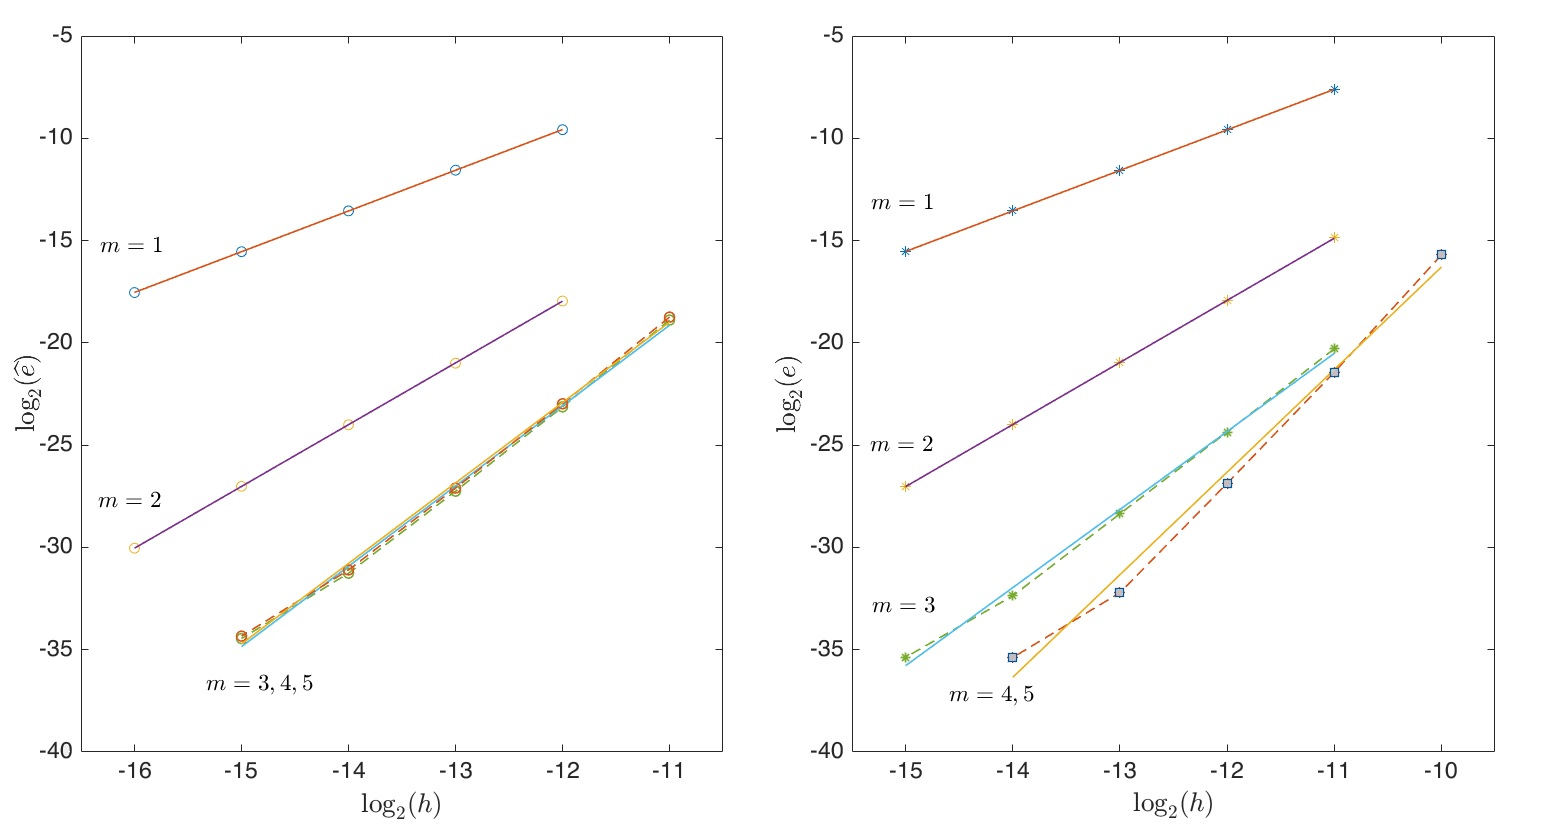
\includegraphics[scale=0.45]{Graphics/lldp/m-plots.jpg}
		\caption{Gráficos Log-log de los errores $\widehat{e}_i=\max_{t_n\in(t)_{h_i}}\nnnorm{\widehat{y}_n-x(t_n)}_\infty$ y $e_i=\max_{t_n\in(t)_{h_i}}\nnnorm{y_n-x(t_n)}_\infty$ contra $h_i$ en al integración del ejemplo \ref{ex:Brus} con las fórmulas (\ref{LLDPK scheme}), $\pf=6$, $\mf=1,2,3,4,5$ and $h_i=2^{-i}$, $i=10,11,12,13,14,15,16$.}
		\label{fig:num-exp-lldp-fix-step:Fig3}
	\end{center}
\end{figure}

\begin{table}[h]
	\centering
	\caption{
        Orden de convergencia $r$ de las fórmulas (\ref{LLDPK scheme}) y su estimado  $\widetilde{r}$ para diferentes valores de $\mf$, los $90\%$ límites de confianza $\Delta$ de $\widetilde {r}$, el coeficiente de determinación $R^2$ de la línea ajustada en la Figura \ref{fig:num-exp-lldp-fix-step:Fig3}.\newline }
		\begin{tabular}{ c  c c c c  c  c c c c}
			\hline
			& \multicolumn{4}{c}{$\widehat{y}$} & & \multicolumn{4}{c}{$y$} \\
			\cline{2-5} \cline{7-10}
			$\mf$ & $r$ & $\widetilde{r}$ & $\pm\varDelta$ & $R^2$ & & $r$ & $\widetilde{r}$ & $\pm\varDelta$ & $R^2$ \\
			\hline
			1 & 2 & 1.99 & 0.01 & 0.99 & & 2 & 1.98 & 0.01 & 0.99 \\
			2 & 3 & 3.02 & 0.01 & 0.99 & & 3 & 3.04 & 0.01 & 0.99 \\
			3 & 4 & 3.93 & 0.20 & 0.99 & & 4 & 3.82 & 0.20 & 0.99 \\
			4 & 4 & 3.93 & 0.19 & 0.99 & & 5 & 5.02 & 0.45 & 0.99 \\
			5 & 4 & 3.93 & 0.19 & 0.99 & & 5 & 5.01 & 0.47 & 0.99 \\
			\hline
		\end{tabular}
	\label{tab:num-exp-lldp-fix-step:morders}
\end{table}

\begin{figure}[h]
	\begin{center}
		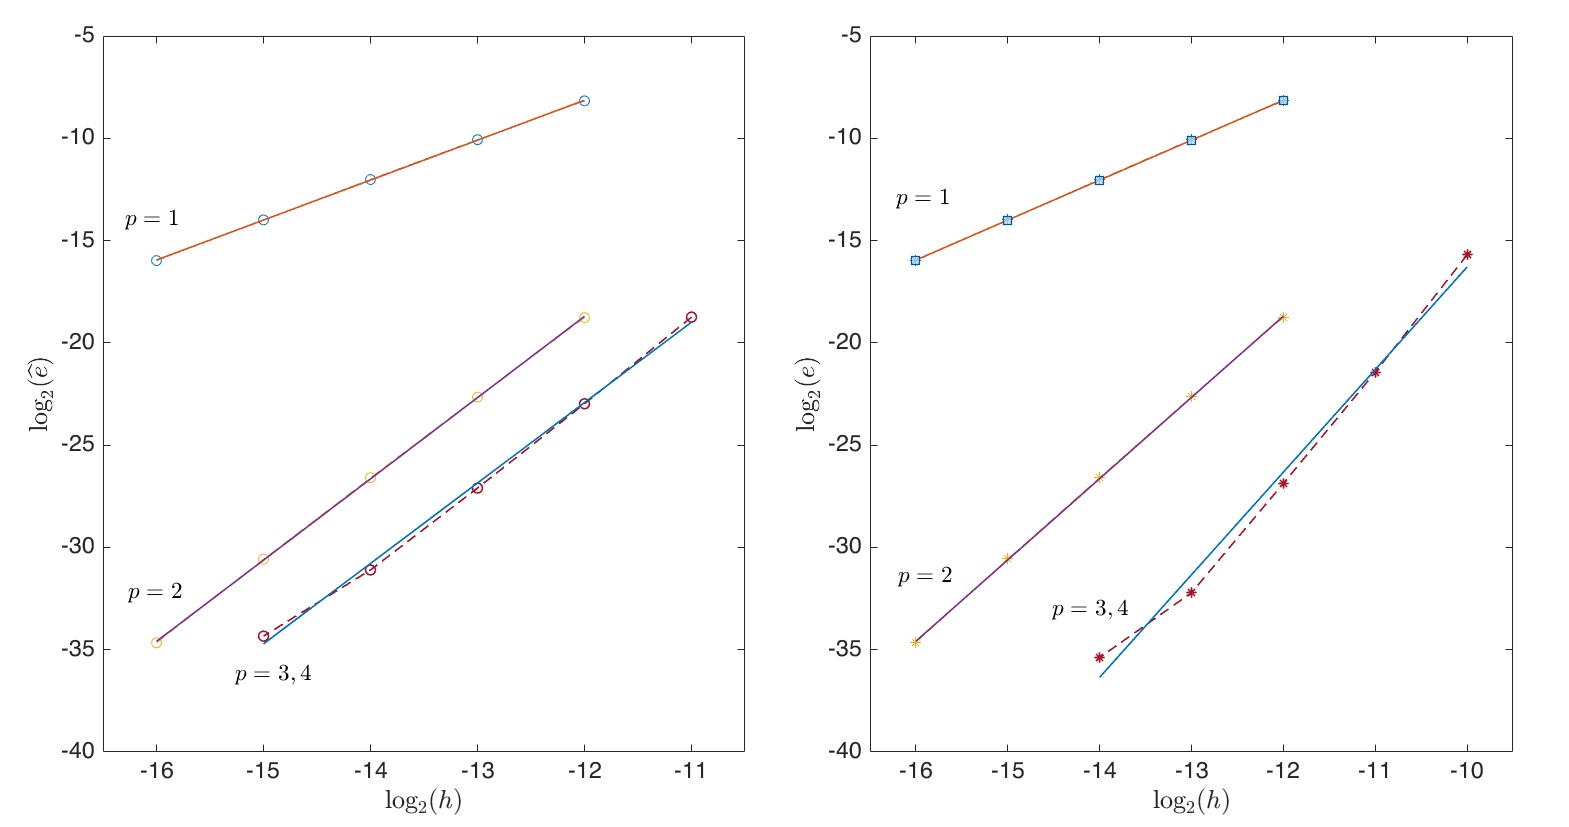
\includegraphics[scale=0.45]{Graphics/lldp/p-plots.jpg}
		\caption{Gráficos Log-log de los errores $\widehat{e}_i=\max_{t_n\in(t)_{h_i}}\nnnorm{\widehat{y}_n-x(t_n)}_\infty$ and $e_i=\max_{t_n\in(t)_{h_i}}\nnnorm{y_n-x(t_n)}_\infty$ contra $h_i$ en al integración del ejemplo \ref{ex:Brus} con las fórmulas (\ref{LLDPK scheme}), $\pf=1,2,3,4$, $\mf=11$ and $h_i=2^{-i}$, $i=10,11,12,13,14,15,16$.}
		\label{fig:num-exp-lldp-fix-step:Fig2}
	\end{center}
\end{figure}


\begin{table}[h]
	\centering
	\caption{
		Orden de convergencia $r$ de las fórmulas (\ref{LLDPK scheme}) y su estimado  $\widetilde{r}$ para diferentes valores de $\pf$, los $90\%$ límites de confianza $\Delta$ de $\widetilde {r}$, el coeficiente de determinación $R^2$ de la línea ajustada en la Figura \ref{fig:num-exp-lldp-fix-step:Fig2}.\newline }
		\begin{tabular}{ c  c c c c  c  c c c c}
			\hline
			& \multicolumn{4}{c}{$\widehat{y}$} & & \multicolumn{4}{c}{$y$} \\
			\cline{2-5} \cline{7-10}
			$\pf+\pf$ & $r$ & $\widetilde{r}$ & $\pm\varDelta$ & $R^2$ & & $r$ & $\widetilde{r}$ & $\pm\varDelta$ & $R^2$ \\
			\hline
			2 & 2 & 1.95 & 0.02 & 0.99 & & 2 & 1.95 & 0.02 & 0.99 \\
			4 & 4 & 3.97 & 0.04 & 0.99 & & 4 & 3.97 & 0.04 & 0.99 \\
			6 & 4 & 3.93 & 0.19 & 0.99 & & 5 & 5.01 & 0.48 & 0.99 \\
			8 & 4 & 3.93 & 0.19 & 0.99 & & 5 & 5.01 & 0.47 & 0.99 \\
			\hline
		\end{tabular}
	\label{tab:num-exp-lldp-fix-step:porders}
\end{table}

\begin{figure}[h]
	\begin{center}
		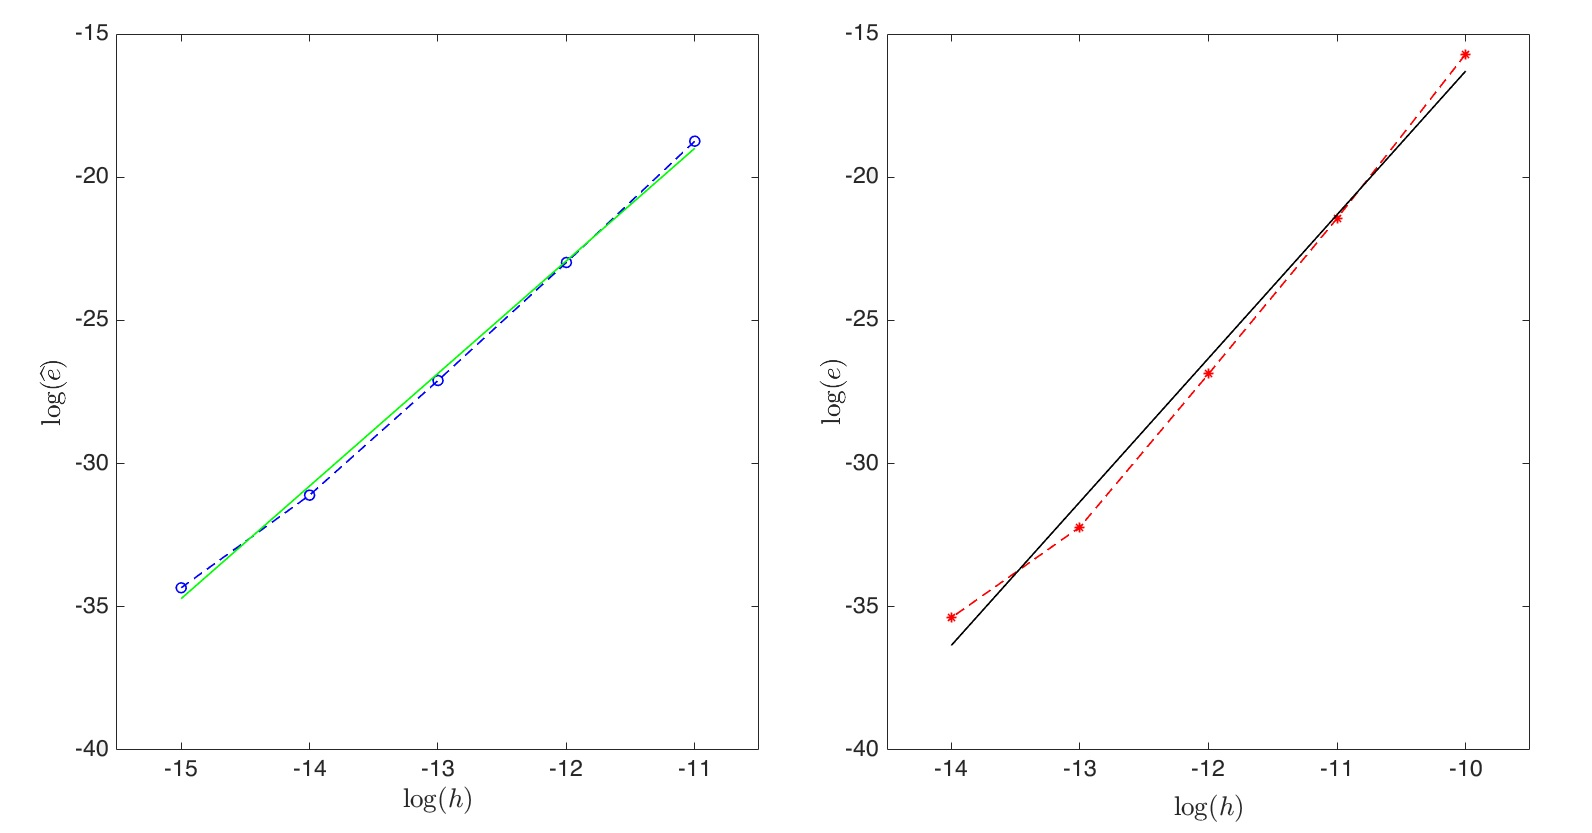
\includegraphics[scale=0.45]{Graphics/lldp/LLDP-plots.jpg}
		\caption{ Gráficos Log-log de los errores $\widehat{e}_i=\max_{t_n\in(t)_{h_i}}\nnnorm{\widehat{y}_n-x(t_n)}_\infty$ y $e_i=\max_{t_n\in(t)_{h_i}}\nnnorm{y_n-x(t_n)}_\infty$ contra $h_i$ en al integración del ejemplo \ref{ex:Brus} con las fórmulas (\ref{LLDPK scheme}), $\pf=6$, $\mf=11$ and $h_i=2^{-i}$, $i=10,11,12,13,14,15$.}
		\label{fig:num-exp-lldp-fix-step:Fig4}
	\end{center}
\end{figure}


\section{Esquemas adaptativos con tamaño de paso variable}

\subsection{Estimación del tamaño de paso}

\subsection{Control del tamaño de paso}

\subsection{Reutilización del Jacobiano}

\subsection{Control del \textit{Breakdown}}

\subsection{Aproximación Krylov-Padé adaptativa}

\subsection{Sketch (renombrar esta sección)}

\subsection{Experimentos numéricos}